% --------------------------------------------------------------------------- %
% --------------------------------------------------------------------------- %
\section{Yields and Significances}
\label{sec:yields}

The observed yield in the search regions is statistically compatible with the predicted background from SM processes. A summary of the total yield in each signal region and predicted background contribution relying only on the techniques described in chapter \ref{ch:bkgs}, referred to as {\it pre-fit} results, is illustrated for each topological region in figure \ref{fig:yieldPrefitTopological}, and the individual yield in each \mttwo bin can be found in figures \ref{fig:yieldPrefit1}, \ref{fig:yieldPrefit2}, and \ref{fig:yieldPrefit3}.
\begin{figure}
	\centering
	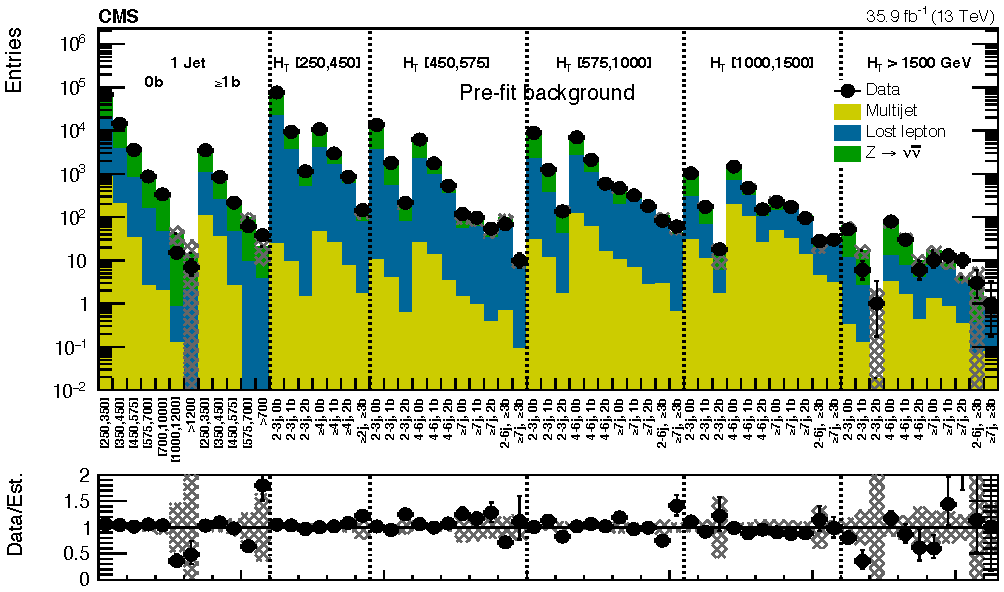
\includegraphics[width=0.95\textwidth]{results/figs/mt2_ALL_fullEstimate}
	\caption{The data yield in each topological region compared to the pre-fit background prediction. The hatched bands illustrate the total uncertainty in the background estimate. Results in the monojet regions are binned in jet \pt, while those in the multijet regions are labeled according to \nj and \nb.}
	\label{fig:yieldPrefitTopological}
\end{figure}
\begin{figure}
	\centering
	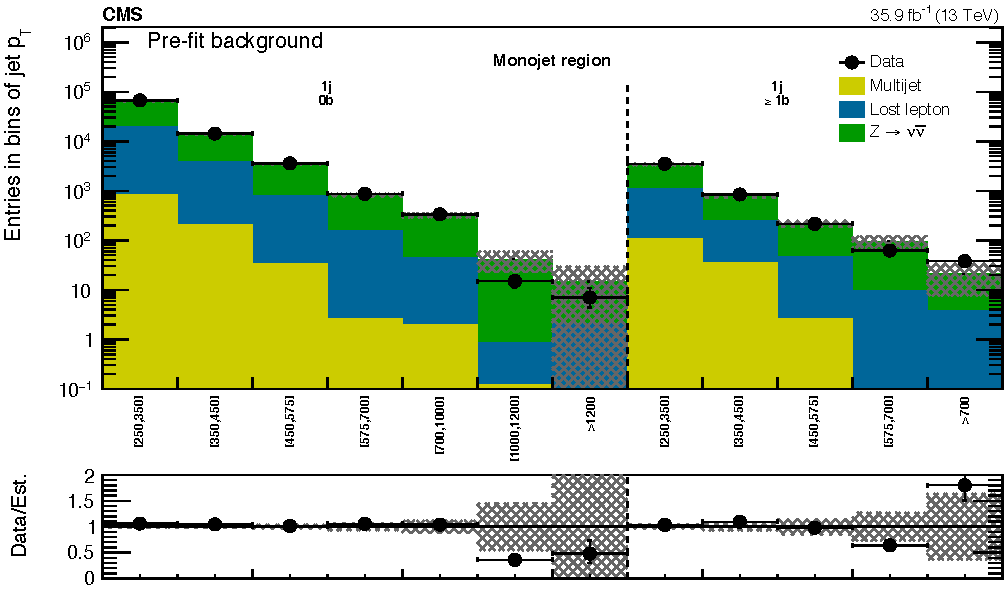
\includegraphics[width=0.95\textwidth]{results/figs/mt2_monojet_fullEstimate}
	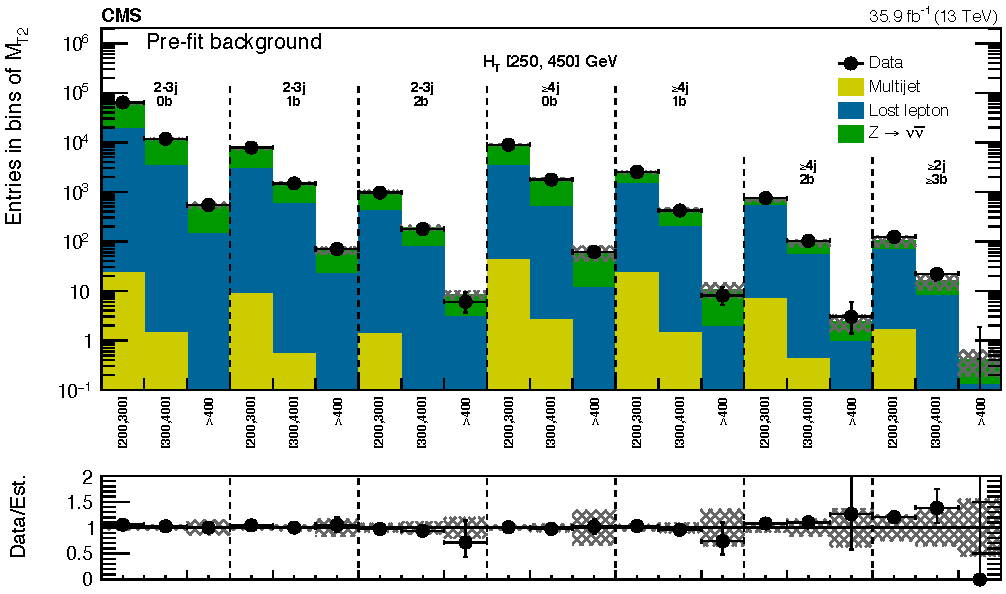
\includegraphics[width=0.95\textwidth]{results/figs/mt2_veryLowHT_fullEstimate}
	\caption{The data yield in the monojet and very-low \HT regions compared to the pre-fit background prediction. The hatched bands illustrate the total uncertainty in the background estimate. Results in the monojet regions are binned in jet \pt in units of GeV, while those in the multijet regions are labeled according to \mttwo bin in units of GeV.}
	\label{fig:yieldPrefit1}
\end{figure}
\begin{figure}
	\centering
	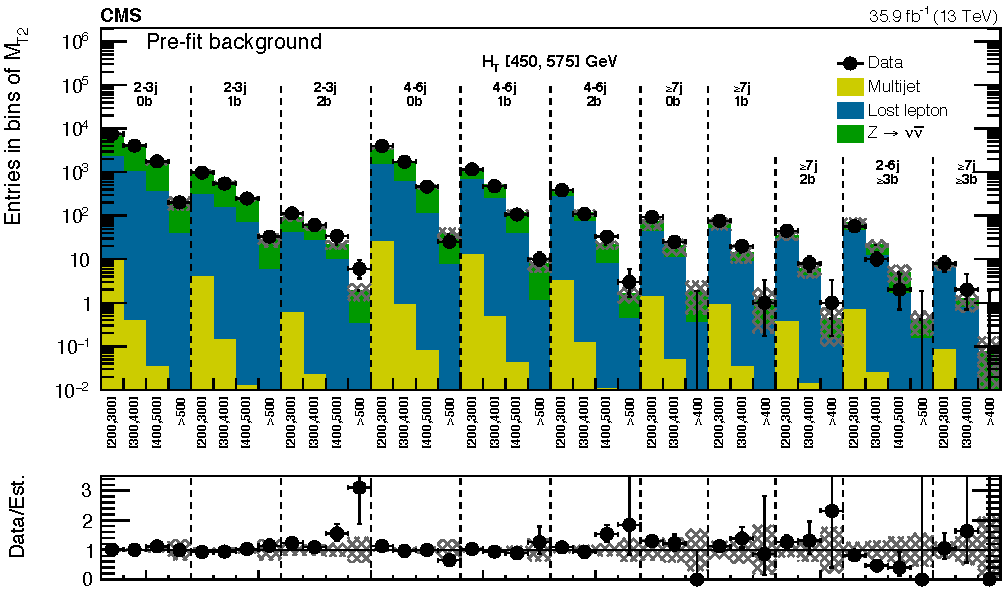
\includegraphics[width=0.95\textwidth]{results/figs/mt2_lowHT_fullEstimate}
	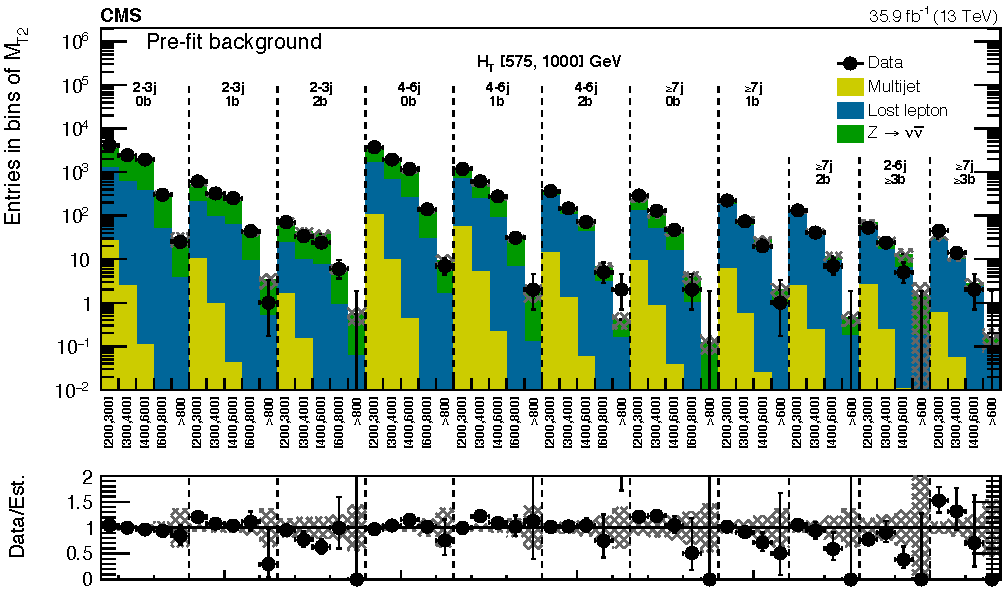
\includegraphics[width=0.95\textwidth]{results/figs/mt2_mediumHT_fullEstimate}
	\caption{The data yield in the low \HT and medium \HT regions compared to the pre-fit background prediction. The hatched bands illustrate the total uncertainty in the background estimate. Results are labeled according to \mttwo bin in units of GeV.}
	\label{fig:yieldPrefit2}
\end{figure}
\begin{figure}
	\centering
	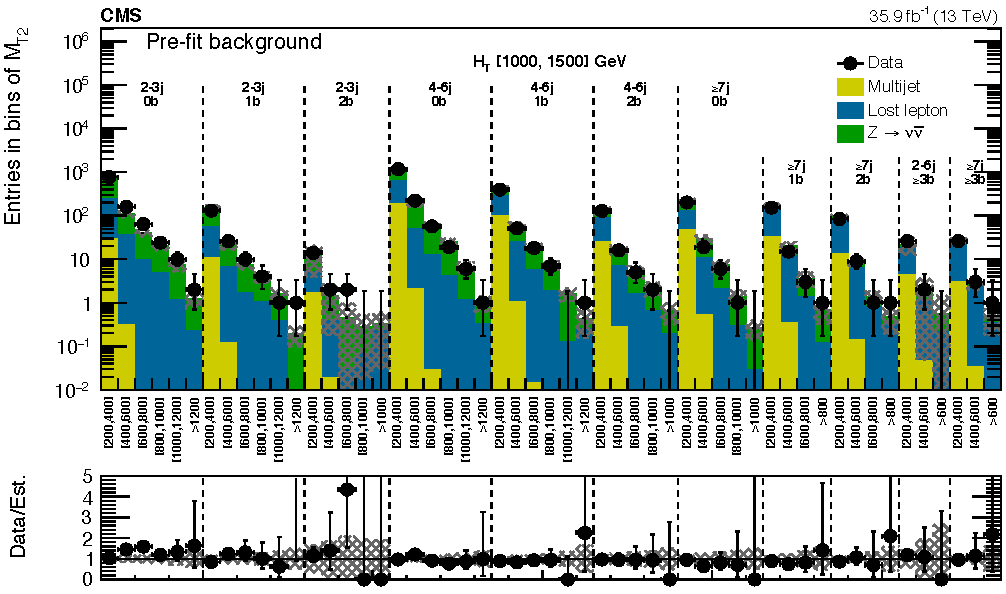
\includegraphics[width=0.95\textwidth]{results/figs/mt2_highHT_fullEstimate}
	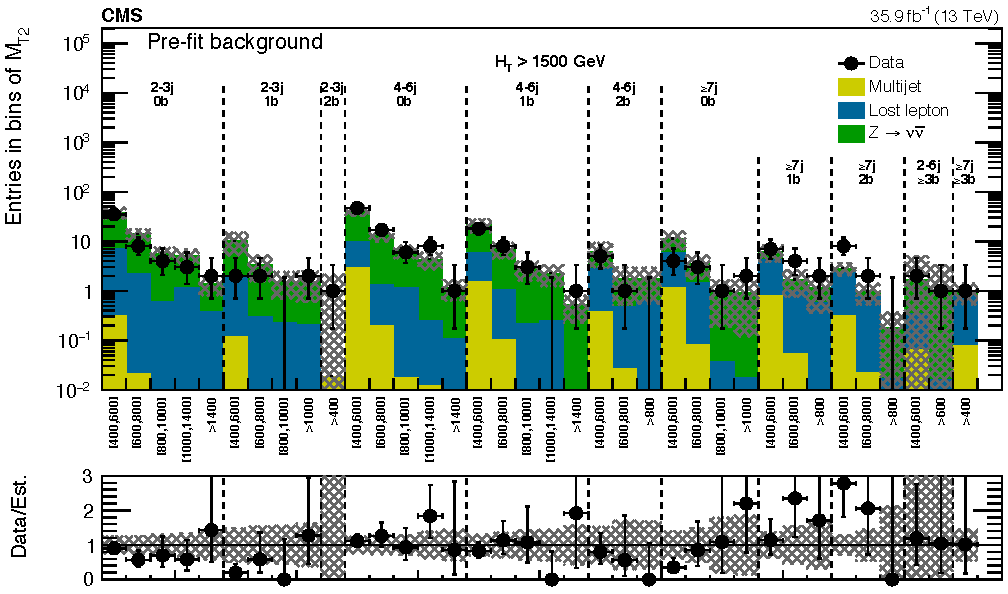
\includegraphics[width=0.95\textwidth]{results/figs/mt2_extremeHT_fullEstimate}
	\caption{The data yield in the high \HT and extreme \HT regions compared to the pre-fit background prediction. The hatched bands illustrate the total uncertainty in the background estimate. Results are labeled according to \mttwo bin in units of GeV.}
	\label{fig:yieldPrefit3}
\end{figure}

The background estimate is further refined by performing a maximum-likelihood fit to data in each signal region, referred to as {\it post-fit} results. The fit is performed using both background-only or background-plus-signal hypotheses to set limits on simplified physics models described in section \ref{sec:interpretations}. The estimates and uncertainties on each background as described in chapter \ref{ch:bkgs} are  used as inputs to the fitting procedure, where the likelihood is constructed as a product of Poisson probability density functions for each signal region with constraints set according to the background uncertainties and signal uncertainties (described in \fm{ref subsection on signal systematics}). The post-fit yield for each topological region is illustrated in figure \ref{fig:yieldPostfitTopological}, and the individual yield in each \mttwo bin can be found in figures \ref{fig:yieldPostfit1}, \ref{fig:yieldPostfit2}, and \ref{fig:yieldPostfit3}. The post-fit procedure has the effect of constraining background and its associated uncertainties when the fitting procedure is applied to data consistent with predictions modeling uncertainties appropriately.
\begin{figure}
	\centering
	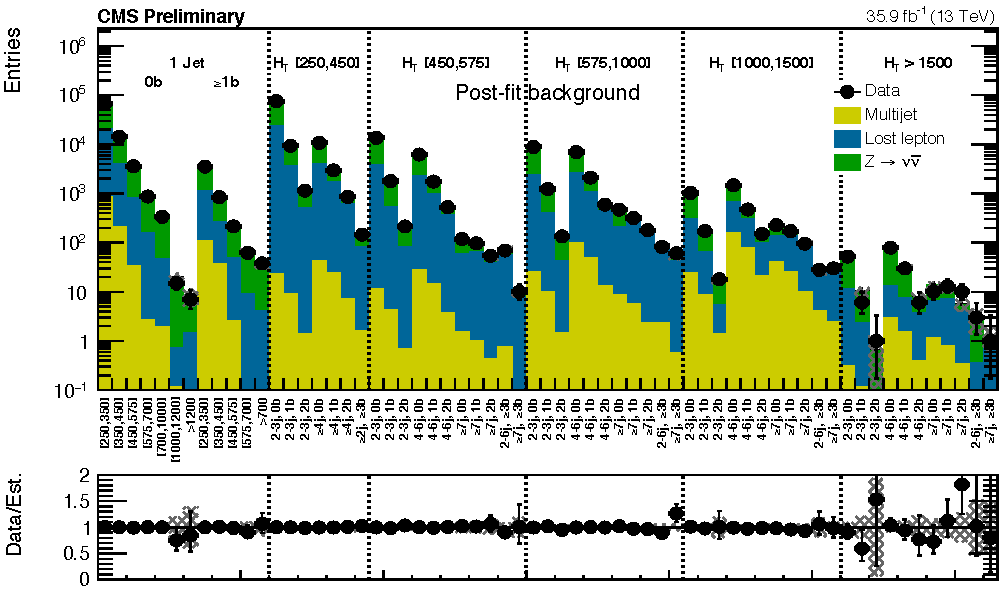
\includegraphics[width=0.95\textwidth]{results/figs/postfit/mt2_ALL_fullEstimate}
	\caption{The data yield in each topological region compared to the post-fit background prediction. The hatched bands illustrate the total uncertainty in the background estimate. Results in the monojet regions are binned in jet \pt, while those in the multijet regions are labeled according to \nj and \nb.}
	\label{fig:yieldPostfitTopological}
\end{figure}
\begin{figure}
	\centering
	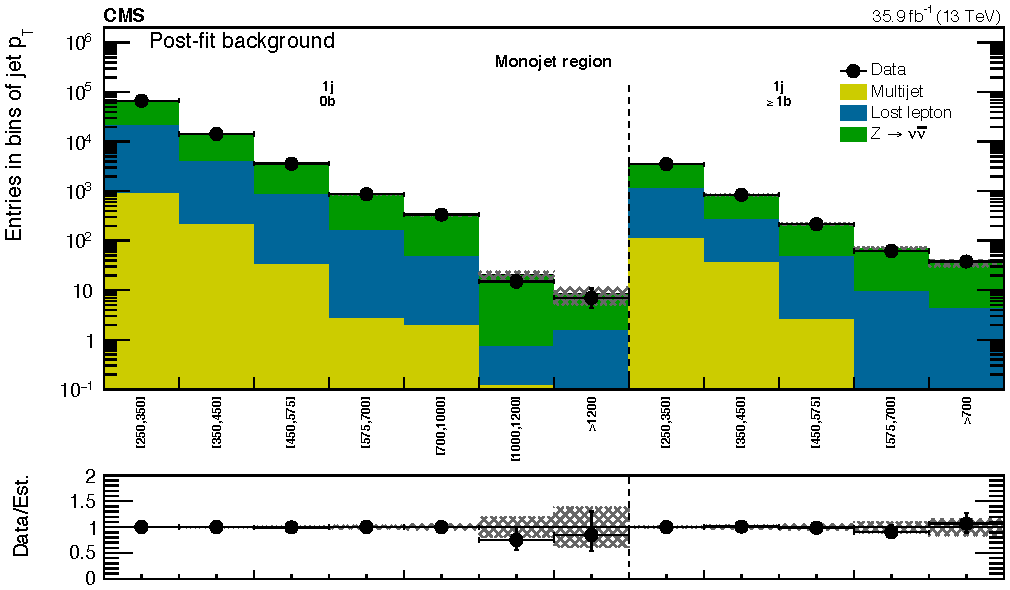
\includegraphics[width=0.95\textwidth]{results/figs/postfit/mt2_monojet_fullEstimate}
	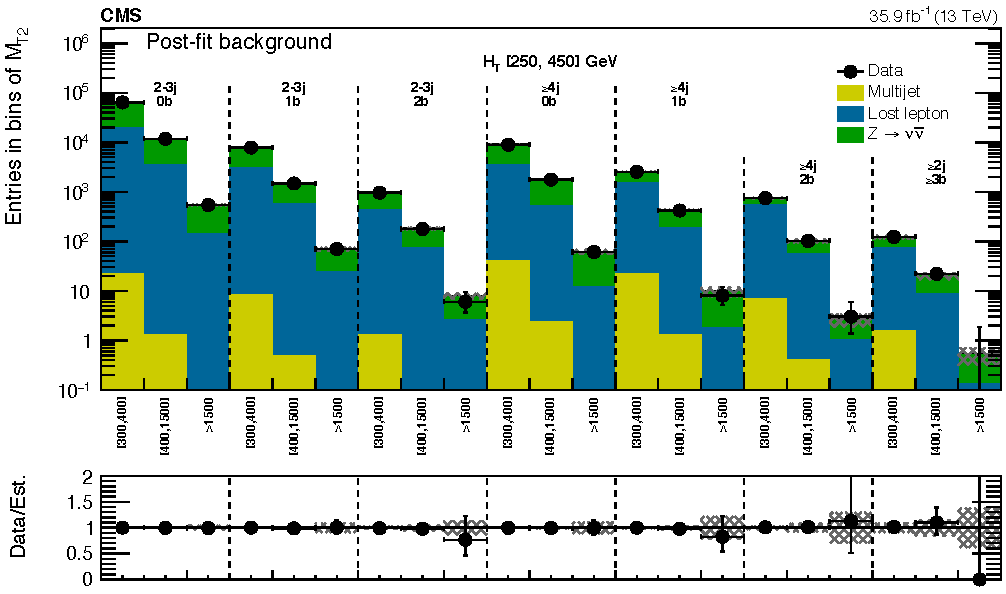
\includegraphics[width=0.95\textwidth]{results/figs/postfit/mt2_veryLowHT_fullEstimate}
	\caption{The data yield in the monojet and very-low \HT regions compared to the post-fit background prediction. The hatched bands illustrate the total uncertainty in the background estimate. Results in the monojet regions are binned in jet \pt in units of GeV, while those in the multijet regions are labeled according to \mttwo bin in units of GeV.}
	\label{fig:yieldPostfit1}
\end{figure}
\begin{figure}
	\centering
	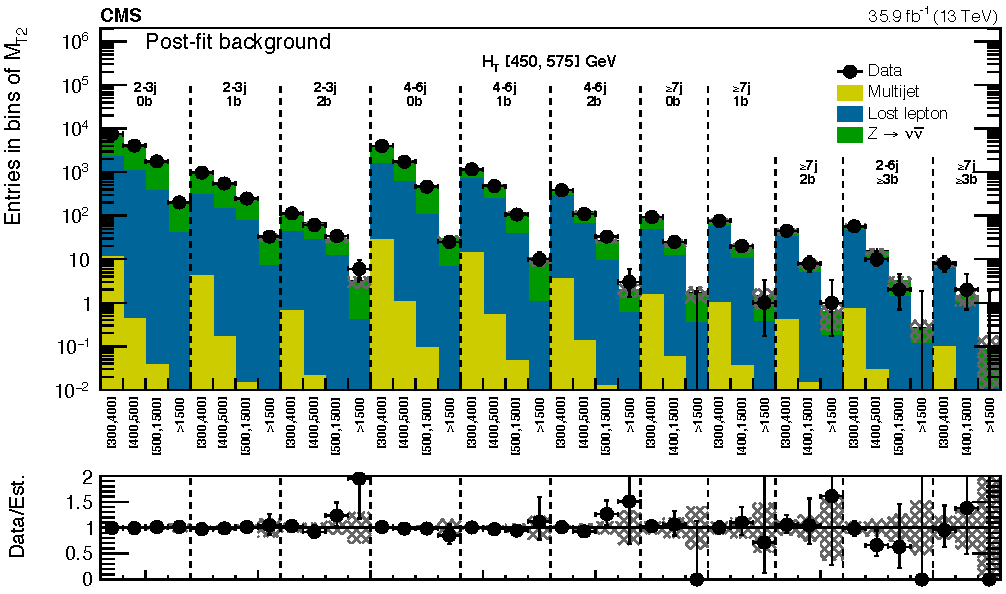
\includegraphics[width=0.95\textwidth]{results/figs/postfit/mt2_lowHT_fullEstimate}
	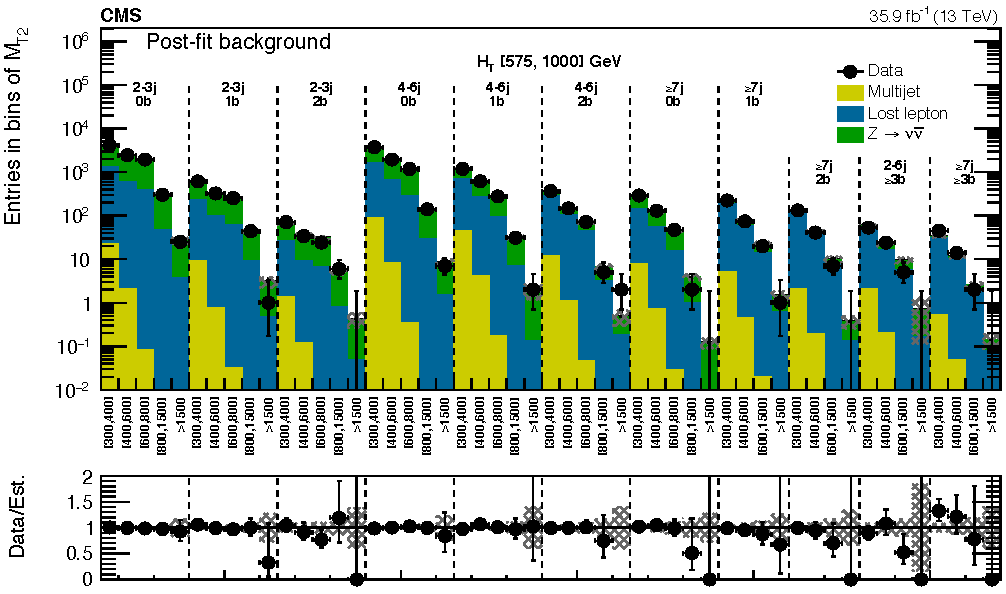
\includegraphics[width=0.95\textwidth]{results/figs/postfit/mt2_mediumHT_fullEstimate}
	\caption{The data yield in the low \HT and medium \HT regions compared to the post-fit background prediction. The hatched bands illustrate the total uncertainty in the background estimate. Results are labeled according to \mttwo bin in units of GeV.}
	\label{fig:yieldPostfit2}
\end{figure}
\begin{figure}
	\centering
	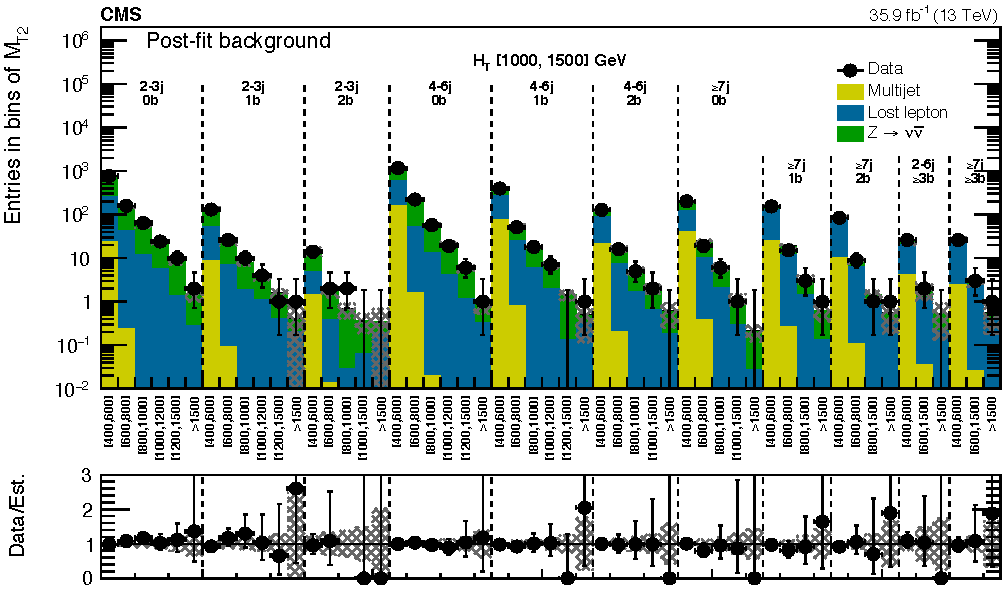
\includegraphics[width=0.95\textwidth]{results/figs/postfit/mt2_highHT_fullEstimate}
	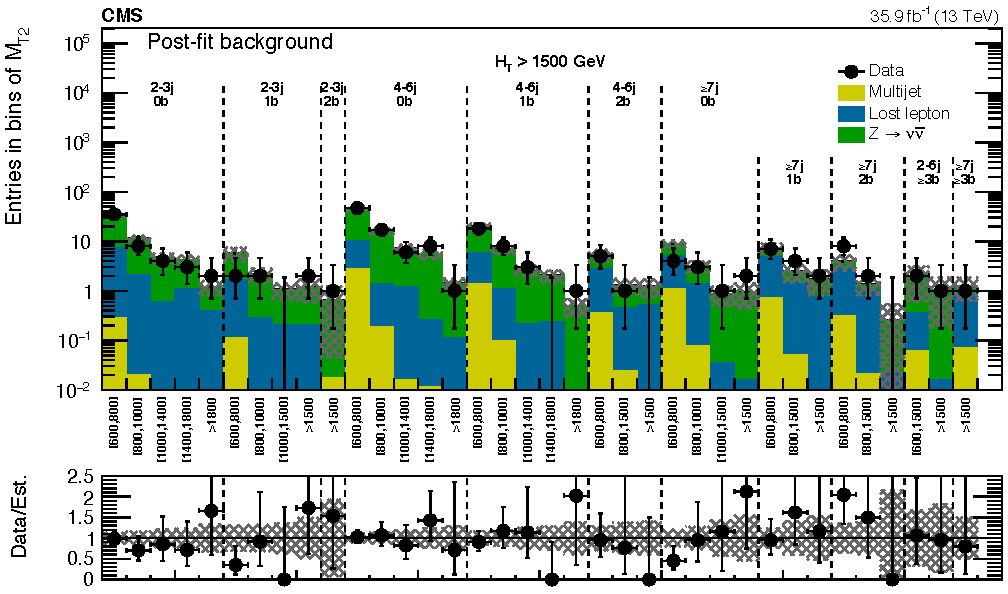
\includegraphics[width=0.95\textwidth]{results/figs/postfit/mt2_extremeHT_fullEstimate}
	\caption{The data yield in the high \HT and extreme \HT regions compared to the post-fit background prediction. The hatched bands illustrate the total uncertainty in the background estimate. Results are labeled according to \mttwo bin in units of GeV.}
	\label{fig:yieldPostfit3}
\end{figure}
% --------------------------------------------------------------------------- %
% --------------------------------------------------------------------------- %
